\chapter{Kristallen I: het perfecte kristal en de metalen}\label{ch:b1:crystals-metals}

Een koperdraad kan dunner dan een haar worden getrokken zonder te breken;
een brok zout spat onder een hamer uiteen. Een smid verhit een staaf ijzer
tot ze gloeit, smeedt ze, dompelt ze in water, en de staaf komt er veel
harder uit dan ze erin ging. Het verschil tussen die gedragingen zit in de
manier waarop de atomen in de vaste stof gestapeld zijn. De meeste vaste
stoffen zijn \omterm{def:b1:crystals-metals:crystal}{kristallen}: hun atomen zitten op een patroon dat zich
miljarden keren in elke richting identiek herhaalt. Dit hoofdstuk
beschrijft zulke patronen, telt hun atomen, meet hoe dicht ze gepakt zijn
en waar de holten tussen hen liggen, en gebruikt het resultaat om metalen
en legeringen te begrijpen. Het volgende hoofdstuk past dezelfde
werktuigen toe op ionaire, covalente en moleculaire vaste stoffen.

\begin{recall}
Metalen staan hun \omterm{def:b1:quantum-numbers:configuration}{valentie-elektronen} gemakkelijk af: ze hebben lage
ionisatie-energieën en \omterm{def:b1:periodicity:electronegativity}{elektronegativiteiten} (\cref{ch:b1:periodicity}).
Atoomstralen werden gedefinieerd in \cref{def:b1:periodicity:radius}. De
dichtheid, een eigenschap die in de natuurkunde bestudeerd wordt, wordt
als bekend gebruikt: $\rho = m/V$.
\end{recall}

\begin{omfigure}
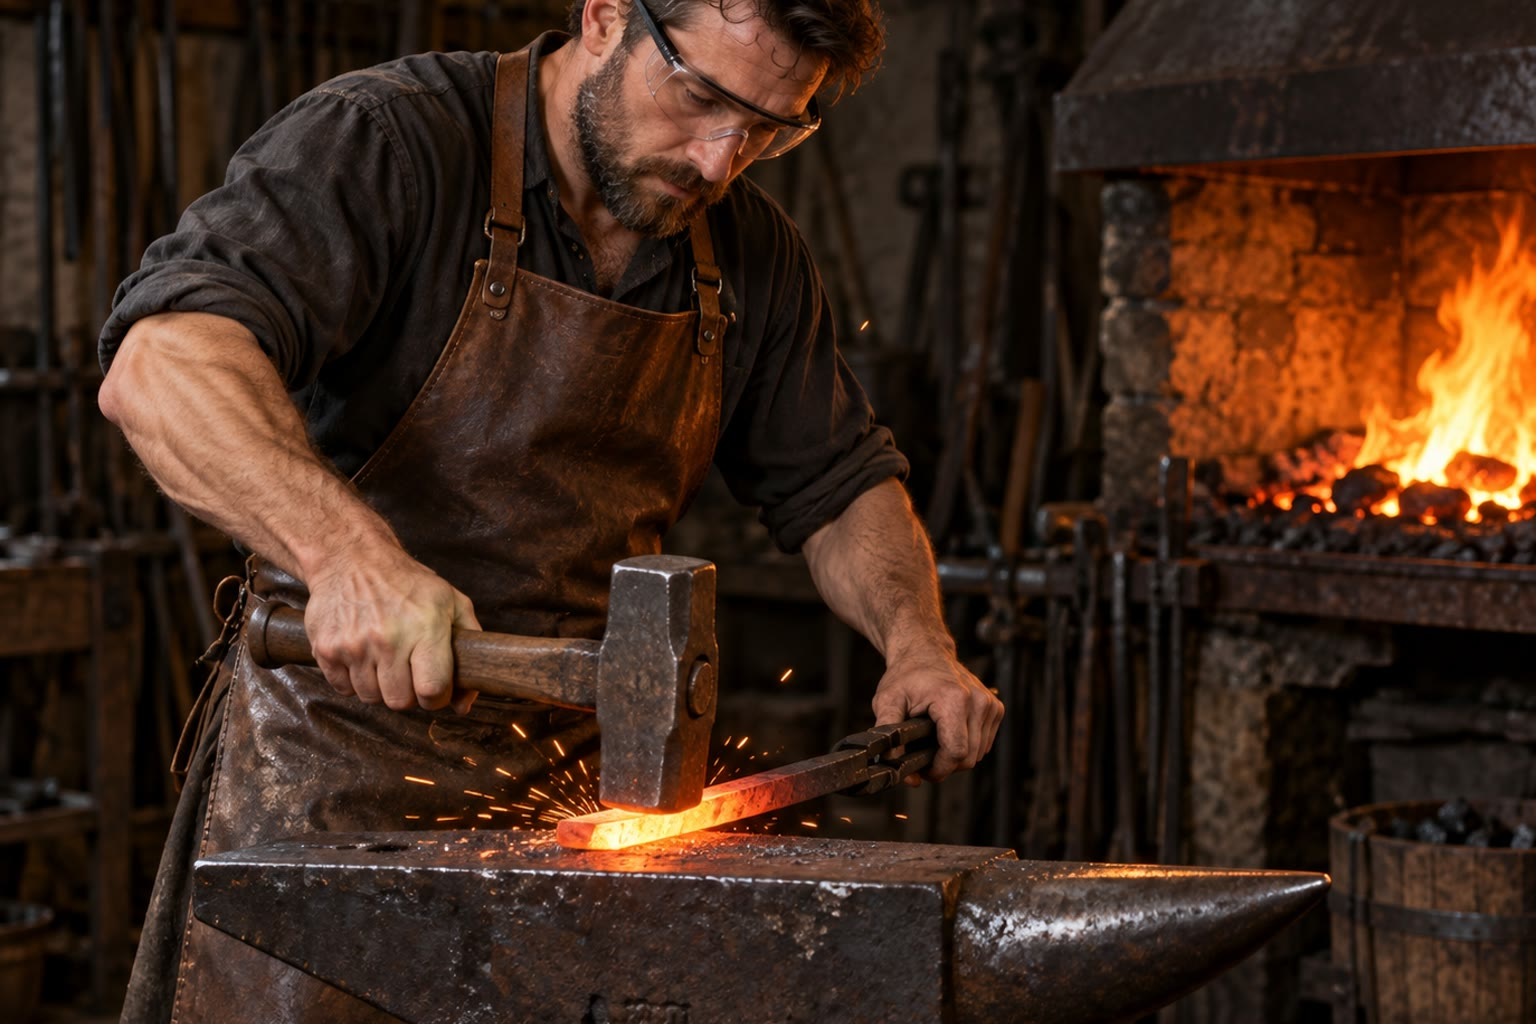
\includegraphics[width=0.55\linewidth]{images/book2/ai/b1-05-blacksmith.jpg}

{\small Een smid die staal smeedt. Oranje gloeiend ijzer heeft een andere
kristalstructuur dan ijzer bij kamertemperatuur, en kan meer koolstof
opnemen (weekendprobleem).}
\end{omfigure}

\section{Het model van het perfecte kristal}

\begin{definition}[Kristal, amorfe vaste stof, perfect kristal]\label{def:b1:crystals-metals:crystal}
Een \emph{kristal}\index{kristal} is een vaste stof waarvan de deeltjes
(atomen, ionen of moleculen) geschikt zijn volgens een patroon dat zich in
drie dimensies periodiek herhaalt. Een vaste stof zonder zo'n orde op
lange afstand is een \emph{amorfe vaste stof}\index{amorfe vaste stof}
(glas, de meeste kunststoffen). Het \emph{model van het perfecte
kristal}\index{model van het perfecte kristal} beschrijft een kristal als
oneindig en zonder defecten: geen ontbrekende of extra atomen, geen
onzuiverheden, geen grenzen.
\end{definition}

\begin{definition}[Rooster, motief, eenheidscel]\label{def:b1:crystals-metals:lattice}
Een \emph{rooster}\index{rooster} is een oneindige verzameling punten, de
\emph{roosterpunten}\index{roosterpunt}, verkregen uit één ervan door alle
translaties $u\,\vec a + v\,\vec b + w\,\vec c$ met gehele $u$, $v$,
$w$. Het \omterm{def:b1:crystals-metals:crystal}{kristal} ontstaat door op elk roosterpunt hetzelfde
\emph{motief}\index{motief} te plaatsen (één atoom, een groep atomen of
ionen). Een \emph{eenheidscel}\index{eenheidscel} is een parallellepipedum
opgespannen door $\vec a$, $\vec b$, $\vec c$ waarvan de translaties de
ruimte vullen; de lengten van de ribben en de hoeken zijn de
\emph{roosterparameters}\index{roosterparameters}
$a$, $b$, $c$, $\alpha$, $\beta$, $\gamma$. In een kubische cel is
$a = b = c$ en zijn de hoeken $90^\circ$.
\end{definition}

\begin{remark}[Echte kristallen]\label{rem:b1:crystals-metals:real}
Echte \omterm{def:b1:crystals-metals:crystal}{kristallen} zijn eindig en onvolmaakt: ze bevatten vacatures,
onzuiverheden, dislocaties en korrelgrenzen, die veel eigenschappen
bepalen (de taaiheid van koper, de hardheid van staal). Die defecten
worden bestudeerd in het deel van jaar 3; het perfecte \omterm{def:b1:crystals-metals:crystal}{kristal} levert de
geometrie, de dichtheid en de \omterm{def:b1:crystals-metals:compactness}{compactheid}, die door defecten nauwelijks
veranderen.
\end{remark}

\begin{definition}[Multipliciteit van een cel]\label{def:b1:crystals-metals:multiplicity}
De \emph{multipliciteit}\index{multipliciteit} $Z$ van een cel is het
aantal motieven (of atomen) dat ertoe behoort, waarbij elk atoom dat met
naburige cellen gedeeld wordt meetelt voor het deel dat binnen de cel
ligt.
\end{definition}

\begin{method}[De atomen van een cel tellen]\label{met:b1:crystals-metals:count}
In een kubische cel wordt een atoom op een hoekpunt gedeeld door 8 cellen
en telt het voor $1/8$; op een ribbe wordt het gedeeld door 4 en telt het
voor $1/4$; op een zijvlak wordt het gedeeld door 2 en telt het voor
$1/2$; binnenin telt het voor 1. Tel de bijdragen op.
\end{method}

\begin{definition}[Coördinatiegetal]\label{def:b1:crystals-metals:coordination}
Het \emph{coördinatiegetal}\index{coordinatiegetal@coördinatiegetal} van
een deeltje in een vaste stof is het aantal naaste buren, de buren op de
kortste afstand.
\end{definition}

\begin{definition}[Compactheid]\label{def:b1:crystals-metals:compactness}
De \emph{compactheid}\index{compactheid} (of pakkingsfractie) van een
\omterm{def:b1:crystals-metals:crystal}{kristal} van harde bollen is de fractie van het volume die door de bollen
wordt ingenomen: voor een cel met volume $V$ die $Z$ bollen met straal
$R$ bevat, is
\[
  C = \frac{Z \cdot \frac43 \pi R^3}{V} .
\]
\end{definition}


\begin{proposition}[Dichtheid uit de cel]\label{prop:b1:crystals-metals:density}
De dichtheid van een \omterm{def:b1:crystals-metals:crystal}{kristal} waarvan de cel, met volume $V$, $Z$ deeltjes
met molaire massa $M$ bevat, is
\[
  \rho = \frac{Z\,M}{N_A\,V} .
\]
\end{proposition}


\begin{proof}
De cel bevat $Z$ deeltjes, met massa $Z\,M/N_A$; het \omterm{def:b1:crystals-metals:crystal}{kristal} is de
herhaalde cel, dus zijn dichtheid is die van één cel.
\end{proof}

\section{Dichtste stapelingen: kubisch vlakgecentreerd en hexagonaal}

\begin{definition}[Dichtste stapeling, FCC, HCP]\label{def:b1:crystals-metals:packings}
Een \emph{dichtste stapeling}\index{dichtste stapeling} van identieke
bollen wordt opgebouwd uit dicht gepakte lagen, waarin elke bol zes
andere raakt, zo gestapeld dat elke bol van een laag in een holte van de
laag eronder ligt. De stapeling $ABCABC\dots$ geeft de \emph{kubisch
vlakgecentreerde structuur}\index{kubisch vlakgecentreerde structuur}
(FCC, of kubisch dichtste stapeling); de stapeling $ABAB\dots$ geeft de
\emph{hexagonaal dichtste stapeling}\index{hexagonaal dichtste stapeling}
(HCP). Een derde, niet dichtst gestapelde structuur van metalen is de
\emph{kubisch ruimtegecentreerde structuur}\index{kubisch ruimtegecentreerde structuur}
(BCC), een kubus met één atoom op elk hoekpunt en één in het midden.
\end{definition}

\begin{omfigure}
\begin{tikzpicture}[font=\small]
  % layer A
  \foreach \i in {0,...,4} \foreach \j in {0,...,3} {
    \pgfmathsetmacro\x{\i+0.5*\j}
    \pgfmathsetmacro\y{0.866*\j}
    \draw[black!60, fill=omDef!25] (\x,\y) circle (0.5);
  }
  % layer B, in the hollows pointing up
  \foreach \i/\j in {1/0, 2/0, 3/0, 1/1, 2/1, 3/1, 1/2, 2/2} {
    \pgfmathsetmacro\x{\i+0.5*\j}
    \pgfmathsetmacro\y{0.866*\j+0.577}
    \draw[omThm!80!black, fill=omThm!25, fill opacity=0.75] (\x,\y) circle (0.5);
  }
  % C positions
  \foreach \i/\j in {1/0, 2/0, 3/0, 1/1, 2/1, 3/1} {
    \pgfmathsetmacro\x{\i+0.5+0.5*\j}
    \pgfmathsetmacro\y{0.866*\j+0.289}
    \fill[omMeth] (\x,\y) circle (0.11);
  }
  \node[anchor=west, align=left] at (6.6,1.6) {A: eerste laag (blauw)\\B: tweede laag, in de\\\phantom{B: }holten van A (rood)\\C: de andere holten\\\phantom{C: }(groene stippen)};
\end{tikzpicture}

{\small Twee dicht gepakte lagen, van bovenaf gezien. Een derde laag kan
boven de holten C liggen (stapeling $ABC$, \omterm{def:b1:crystals-metals:packings}{kubisch vlakgecentreerd}) of
boven de atomen van A (stapeling $AB$, \omterm{def:b1:crystals-metals:packings}{hexagonaal dichtste stapeling}).}
\end{omfigure}

\begin{proposition}[Kubisch vlakgecentreerd]\label{prop:b1:crystals-metals:fcc}
In de FCC-structuur bezetten de atomen de acht hoekpunten en de zes
middelpunten van de zijvlakken van een kubus met ribbe $a$. Dan is
$Z = 4$, is het \omterm{def:b1:crystals-metals:coordination}{coördinatiegetal} 12, raken de atomen elkaar langs een
zijvlakdiagonaal, $a\sqrt2 = 4R$, en is de \omterm{def:b1:crystals-metals:compactness}{compactheid}
\[
  C = \frac{\pi}{3\sqrt2} \approx 0.74 .
\]
\end{proposition}

\begin{proof}
$Z = 8 \times \frac18 + 6 \times \frac12 = 4$. Een atoom in het midden
van een zijvlak raakt de vier hoekpunten van zijn zijvlak en de vier
zijvlakmiddelpunten van elk van de twee cellen die het zijvlak delen:
$4 + 4 + 4 = 12$ buren op $a\sqrt2/2$. Op een zijvlakdiagonaal, met
lengte $a\sqrt2$, liggen een hoekatoom, een zijvlakatoom en een hoekatoom
die elkaar raken: $a\sqrt2 = 4R$. Dan is
$C = 4 \cdot \frac43\pi R^3/a^3 = \frac{16}{3}\pi R^3/(2\sqrt2 R)^3 \cdot
\frac{1}{1} = \frac{16\pi}{3 \times 16\sqrt2} = \frac{\pi}{3\sqrt2}$.
\end{proof}

\begin{omfigure}
\tdplotsetmaincoords{60}{100}
\begin{tikzpicture}[tdplot_main_coords, font=\small]
  \pic {omcubeo={3}};
  \node[cellA=6mm] at (0,0,0) {};
  \node[cellA=6mm] at (0,3,0) {};
  \node[cellA=6mm, ball color=omDef!55] at (0,1.5,1.5) {};
  \node[cellA=6mm] at (0,0,3) {};
  \node[cellA=6mm, ball color=omDef!55] at (1.5,1.5,0) {};
  \node[cellA=6mm] at (0,3,3) {};
  \node[cellA=6mm, ball color=omDef!55] at (1.5,0,1.5) {};
  \node[cellA=6mm, ball color=omDef!55] at (1.5,3,1.5) {};
  \node[cellA=6mm] at (3,0,0) {};
  \node[cellA=6mm, ball color=omDef!55] at (1.5,1.5,3) {};
  \node[cellA=6mm] at (3,3,0) {};
  \node[cellA=6mm, ball color=omDef!55] at (3,1.5,1.5) {};
  \node[cellA=6mm] at (3,0,3) {};
  \node[cellA=6mm] at (3,3,3) {};
  \draw[omThm, thick] (3,0,0) -- (3,3,3);
\end{tikzpicture}
\hspace{1.2cm}
\begin{tikzpicture}[tdplot_main_coords, font=\small]
  \pic {omcubeo={3}};
  \node[cellA=7mm] at (0,0,0) {};
  \node[cellA=7mm] at (0,3,0) {};
  \node[cellA=7mm] at (0,0,3) {};
  \node[cellA=7mm] at (0,3,3) {};
  \node[cellA=7mm, ball color=omDef!55] at (1.5,1.5,1.5) {};
  \node[cellA=7mm] at (3,0,0) {};
  \node[cellA=7mm] at (3,3,0) {};
  \node[cellA=7mm] at (3,0,3) {};
  \node[cellA=7mm] at (3,3,3) {};
  \draw[omThm, thick] (3,0,0) -- (0,3,3);
\end{tikzpicture}

{\small Links: de \omterm{def:b1:crystals-metals:packings}{kubisch vlakgecentreerde} cel (hoekatomen grijs,
zijvlakatomen blauw). De atomen raken elkaar langs een zijvlakdiagonaal
(rode lijn, $a\sqrt2 = 4R$). Rechts: de \omterm{def:b1:crystals-metals:packings}{kubisch ruimtegecentreerde} cel;
de atomen raken elkaar langs de lichaamsdiagonaal (rode lijn,
$a\sqrt3 = 4R$). De atomen zijn voor de duidelijkheid kleiner getekend
dan hun contactgrootte.}
\end{omfigure}

\begin{proposition}[Hexagonaal dichtste stapeling]\label{prop:b1:crystals-metals:hcp}
In de HCP-structuur bevat het conventionele hexagonale prisma, met
grondribbe $a$ en hoogte $c$, 6 atomen; het \omterm{def:b1:crystals-metals:coordination}{coördinatiegetal} is 12; voor
bollen die elkaar raken is $a = 2R$, $c/a = \sqrt{8/3} \approx 1.633$, en
de \omterm{def:b1:crystals-metals:compactness}{compactheid} is dezelfde als bij FCC, $\pi/(3\sqrt2) \approx 0.74$.
\end{proposition}

\begin{proof}
Het prisma heeft 12 hoekatomen gedeeld door 6 prisma's, 2 atomen in het
midden van de grondvlakken gedeeld door 2, en 3 atomen binnenin:
$12/6 + 2/2 + 3 = 6$. Elk atoom raakt zes buren in zijn laag en drie in
elke aangrenzende laag: 12. Een atoom van laag B ligt op drie elkaar
rakende atomen van laag A en vormt er een regelmatige tetraëder met ribbe
$2R$ mee, met hoogte $2R\sqrt{2/3}$; twee lagen verder is
$c = 4R\sqrt{2/3}$, dus $c/a = 2\sqrt{2/3} = \sqrt{8/3}$. Het volume van
het prisma is $\frac{3\sqrt3}{2}a^2 c = \frac{3\sqrt3}{2}(2R)^2 \cdot
4R\sqrt{2/3} = 24\sqrt2\,R^3$, en $C = 6 \cdot \frac43\pi R^3/(24\sqrt2
R^3) = \pi/(3\sqrt2)$.
\end{proof}

\begin{omfigure}
\tdplotsetmaincoords{70}{113}
\begin{tikzpicture}[tdplot_main_coords, font=\small, scale=1.25]
  \pic[transform shape] {omhexprismo={1.6}{2.6}};
  \node[cellA=6mm] at (-1.6,0,0) {};
  \node[cellA=6mm] at (-0.8,-1.386,0) {};
  \node[cellA=6mm] at (-1.6,0,2.6) {};
  \node[cellA=6mm] at (-0.8,-1.386,2.6) {};
  \node[cellA=6mm] at (-0.8,1.386,0) {};
  \node[cellA=6mm, ball color=omThm!60] at (-0.8,0.462,1.3) {};
  \node[cellA=6mm] at (0,0,0) {};
  \node[cellA=6mm, ball color=omThm!60] at (0,-0.924,1.3) {};
  \node[cellA=6mm] at (0.8,-1.386,0) {};
  \node[cellA=6mm] at (-0.8,1.386,2.6) {};
  \node[cellA=6mm] at (0,0,2.6) {};
  \node[cellA=6mm] at (0.8,-1.386,2.6) {};
  \node[cellA=6mm] at (0.8,1.386,0) {};
  \node[cellA=6mm, ball color=omThm!60] at (0.8,0.462,1.3) {};
  \node[cellA=6mm] at (1.6,0,0) {};
  \node[cellA=6mm] at (0.8,1.386,2.6) {};
  \node[cellA=6mm] at (1.6,0,2.6) {};
\end{tikzpicture}

{\small Het hexagonale prisma van de \omterm{def:b1:crystals-metals:packings}{dichtste stapeling}, met grondribbe
$a$ (de zijde van de zeshoek) en hoogte $c$: lagen A (grijs) onderaan en
bovenaan, laag B (rood) halverwege, in de holten van A.}
\end{omfigure}

\section{Kubisch ruimtegecentreerd en de metallische elementen}

\begin{proposition}[Kubisch ruimtegecentreerd]\label{prop:b1:crystals-metals:bcc}
In de BCC-structuur is $Z = 2$, is het \omterm{def:b1:crystals-metals:coordination}{coördinatiegetal} 8, raken de
atomen elkaar langs de lichaamsdiagonaal van de kubus, $a\sqrt3 = 4R$, en
is de \omterm{def:b1:crystals-metals:compactness}{compactheid}
\[
  C = \frac{\pi\sqrt3}{8} \approx 0.68 .
\]
\end{proposition}


\begin{proof}
$Z = 8 \times \frac18 + 1 = 2$. Het centrale atoom raakt de acht
hoekatomen: de lichaamsdiagonaal $a\sqrt3$ bevat een hoekatoom, het
centrale atoom en een hoekatoom, $a\sqrt3 = 4R$. Dan is $C = 2 \cdot \frac43\pi R^3/a^3 =
\frac83\pi R^3 (\sqrt3/(4R))^3 = \frac83\pi \cdot \frac{3\sqrt3}{64} =
\frac{\pi\sqrt3}{8}$.
\end{proof}

\begin{proposition}[De dichtste stapeling is de dichtste]\label{prop:b1:crystals-metals:kepler}
Geen enkele stapeling van identieke bollen heeft een grotere \omterm{def:b1:crystals-metals:compactness}{compactheid}
dan $\pi/(3\sqrt2) \approx 0.7405$, de waarde van FCC en HCP.
\end{proposition}
\admitted

\begin{history}[Het vermoeden van Kepler, 1611--2017]
In een kort essay over sneeuwvlokken, geschreven in 1611, beweerde
Johannes Kepler dat geen enkele manier om kanonskogels op te stapelen
dichter kon zijn dan de piramide van de kruidenier, de \omterm{def:b1:crystals-metals:packings}{kubisch
vlakgecentreerde} stapeling. De bewering weerstond bijna vier eeuwen elk
bewijs. Thomas Hales gaf in 1998 een bewijs met hulp van de computer, en
een formeel bewijs dat regel voor regel door een computer werd
gecontroleerd, werd in 2014 voltooid en in 2017 gepubliceerd.
\end{history}

\begin{example}[Drie metalen]\label{ex:b1:crystals-metals:metals}
Koper is FCC met $a = \qty{361.5}{pm}$: $R = a\sqrt2/4 =
\qty{127.8}{pm}$ en $\rho = 4 \times 63.55/(6.022 \times 10^{23} \times
(3.615 \times 10^{-8})^3) = \qty{8.93}{g/cm^3}$, de gemeten dichtheid.
IJzer bij kamertemperatuur ($\alpha$-ijzer) is BCC met
$a = \qty{286.7}{pm}$: $R = \qty{124.1}{pm}$, $\rho = \qty{7.87}{g/cm^3}$.
Magnesium is HCP met $a = \qty{320.9}{pm}$ en $c = \qty{521.0}{pm}$:
$c/a = 1.624$, dicht bij de ideale $1.633$; zink, met $c/a = 1.856$, is
een uitgerekte hexagonale stapeling.
% ledger: lat:Cu, rho:Cu, lat:Fe-alpha, rho:Fe, lat:Mg.a, lat:Mg.c,
% lat:Zn.a, lat:Zn.c, aw:Cu, aw:Fe, const:NA
\end{example}

\begin{center}
\small
\begin{tabular}{lllccc}
\hline
metaal & structuur & $a$ (pm) & $R$ (pm) & $\rho$ berekend & $\rho$ gemeten \\
\hline
aluminium & FCC & 405.0 & 143.2 & 2.70 & 2.70 \\
koper & FCC & 361.5 & 127.8 & 8.93 & 8.93 \\
zilver & FCC & 408.6 & 144.5 & 10.50 & 10.50 \\
natrium & BCC & 429.1 & 185.8 & 0.967 & 0.97 \\
$\alpha$-ijzer & BCC & 286.7 & 124.1 & 7.87 & 7.87 \\
wolfraam & BCC & 316.5 & 137.0 & 19.26 & 19.3 \\
\hline
\end{tabular}
\end{center}
% ledger: lat:Al, lat:Cu, lat:Ag, lat:Na, lat:Fe-alpha, lat:W, rho:Al,
% rho:Cu, rho:Ag, rho:Na, rho:Fe, rho:W (densities in g/cm3)

\begin{omfigure}
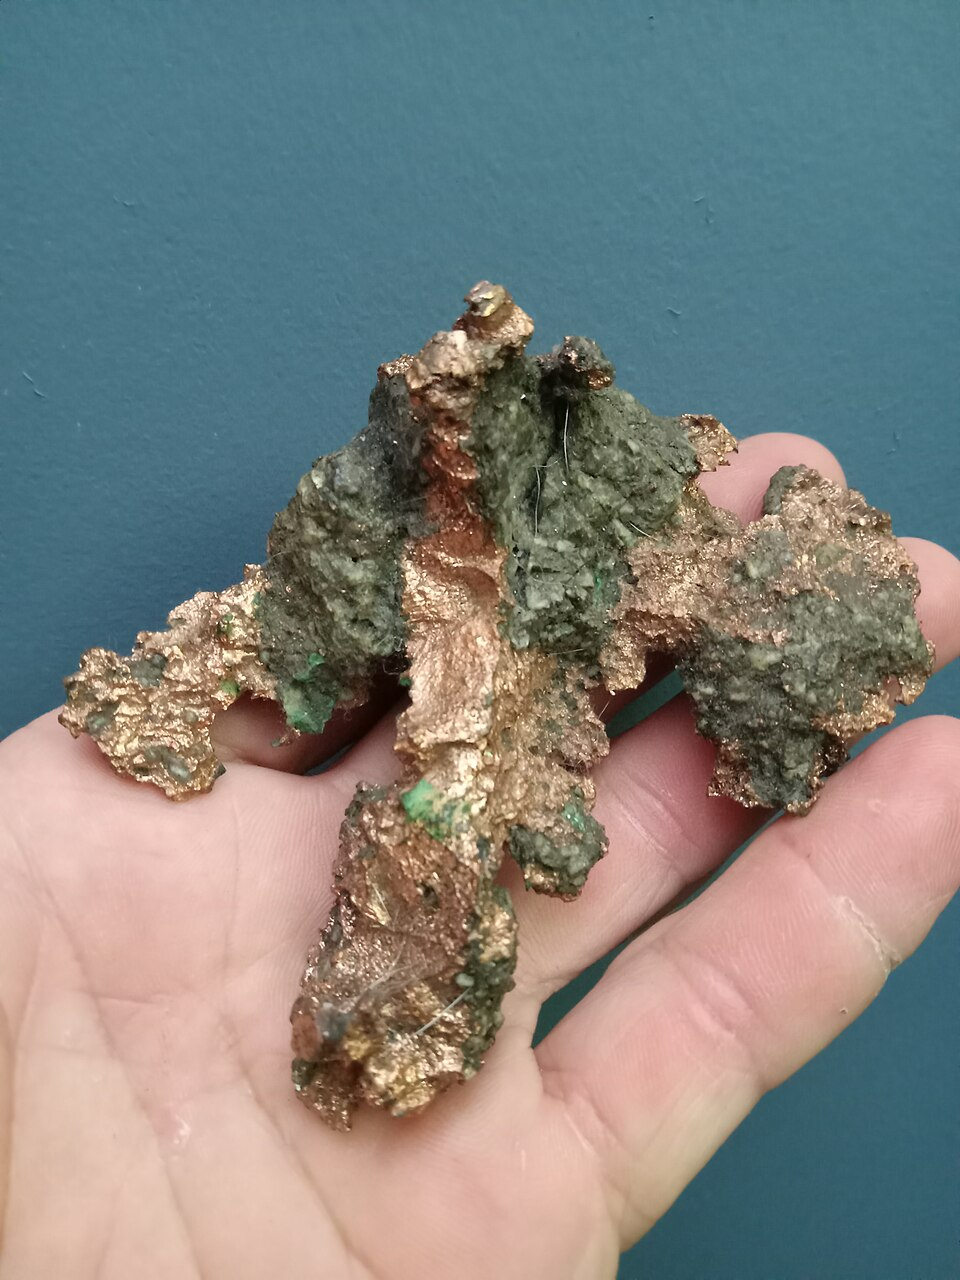
\includegraphics[width=0.36\linewidth]{images/book2/native-copper.jpg}

{\small Een stuk gedegen koper. De vertakte vormen zijn als \omterm{def:b1:crystals-metals:crystal}{kristallen}
gegroeid; het metaal eronder is een mozaïek van FCC-korrels.
Foto: CC0 (Wikimedia Commons).}
\end{omfigure}

\section{Interstitiële holten}

\begin{definition}[Interstitiële holten]\label{def:b1:crystals-metals:site}
Een \emph{interstitiële holte}\index{interstitiele holte@interstitiële holte}
is een ruimte tussen de atomen van een \omterm{def:b1:crystals-metals:crystal}{kristal} waarin een kleiner atoom
kan zitten. Een \emph{tetraëdrische
holte}\index{tetraedrische holte@tetraëdrische holte} ligt in het midden
van een tetraëder van vier atomen, een \emph{octaëdrische
holte}\index{octaedrische holte@octaëdrische holte} in het midden van een
octaëder van zes. De \emph{holtestraal}\index{holtestraal} van een holte
is de straal van de grootste bol die erin past zonder de omringende
atomen uit elkaar te duwen.
\end{definition}

\begin{proposition}[Holten van de FCC-structuur]\label{prop:b1:crystals-metals:sites}
Een FCC-cel bevat 4 \omterm{def:b1:crystals-metals:site}{octaëdrische holten}, in het midden van de kubus en in
het midden van zijn 12 ribben, en 8 \omterm{def:b1:crystals-metals:site}{tetraëdrische holten}, in de
middelpunten van de 8 kleine kubussen met ribbe $a/2$. Voor atomen met
straal $R$ die elkaar raken, zijn de holtestralen
\[
  r_O = (\sqrt2 - 1)R \approx 0.414\,R, \qquad
  r_T = \left(\sqrt{\tfrac32} - 1\right)R \approx 0.225\,R .
\]
\end{proposition}

\begin{proof}
\omterm{def:b1:crystals-metals:site}{Octaëdrische holten}: $1 + 12 \times \frac14 = 4$, evenveel als atomen.
Het midden van de kubus ligt op $a/2$ van de zes zijvlakmiddelpunten:
$r_O + R = a/2$ met $a = 2\sqrt2 R$, dus $r_O = (\sqrt2 - 1)R$.
\omterm{def:b1:crystals-metals:site}{Tetraëdrische holten}: het middelpunt van een kleine kubus met ribbe $a/2$
ligt op een halve lichaamsdiagonaal,
$\frac{a}{2}\cdot\frac{\sqrt3}{2} = \frac{a\sqrt3}{4}$, van de vier atomen
op afwisselende hoekpunten: $r_T + R = \frac{\sqrt3}{4}\,2\sqrt2\,R =
\sqrt{\tfrac32}\,R$.
\end{proof}

\begin{omfigure}
\tdplotsetmaincoords{60}{100}
\begin{tikzpicture}[tdplot_main_coords, font=\small]
  \pic {omcubeo={3}};
  \node[cellA=3.6mm] at (0,0,0) {};
  \node[cellsite=4mm, draw=omThm, fill=omThm!30] at (0,1.5,0) {};
  \node[cellA=3.6mm] at (0,3,0) {};
  \node[cellsite=4mm, draw=omThm, fill=omThm!30] at (0,0,1.5) {};
  \node[cellA=3.6mm] at (0,1.5,1.5) {};
  \node[cellsite=4mm, draw=omThm, fill=omThm!30] at (0,3,1.5) {};
  \node[cellsite=4mm, draw=omThm, fill=omThm!30] at (1.5,0,0) {};
  \node[cellA=3.6mm] at (0,0,3) {};
  \node[cellA=3.6mm] at (1.5,1.5,0) {};
  \node[cellsite=4mm, draw=omThm, fill=omThm!30] at (0,1.5,3) {};
  \node[cellsite=4mm, draw=omThm, fill=omThm!30] at (1.5,3,0) {};
  \node[cellA=3.6mm] at (0,3,3) {};
  \node[cellA=3.6mm] at (1.5,0,1.5) {};
  \node[cellsite=5mm, draw=omThm, fill=omThm!30] at (1.5,1.5,1.5) {};
  \node[cellA=3.6mm] at (1.5,3,1.5) {};
  \node[cellA=3.6mm] at (3,0,0) {};
  \node[cellsite=4mm, draw=omThm, fill=omThm!30] at (1.5,0,3) {};
  \node[cellsite=4mm, draw=omThm, fill=omThm!30] at (3,1.5,0) {};
  \node[cellA=3.6mm] at (1.5,1.5,3) {};
  \node[cellA=3.6mm] at (3,3,0) {};
  \node[cellsite=4mm, draw=omThm, fill=omThm!30] at (1.5,3,3) {};
  \node[cellsite=4mm, draw=omThm, fill=omThm!30] at (3,0,1.5) {};
  \node[cellA=3.6mm] at (3,1.5,1.5) {};
  \node[cellsite=4mm, draw=omThm, fill=omThm!30] at (3,3,1.5) {};
  \node[cellA=3.6mm] at (3,0,3) {};
  \node[cellsite=4mm, draw=omThm, fill=omThm!30] at (3,1.5,3) {};
  \node[cellA=3.6mm] at (3,3,3) {};
  \node[below] at (1.5,1.5,-1.5) {octaëdrische holten (rood)};
\end{tikzpicture}
\hspace{1.2cm}
\begin{tikzpicture}[tdplot_main_coords, font=\small]
  \pic {omcubeo={3}};
  \node[cellA=3.6mm] at (0,0,0) {};
  \node[cellA=3.6mm] at (0,3,0) {};
  \node[cellA=3.6mm] at (0,1.5,1.5) {};
  \node[cellsite=4mm, fill=omDef!30] at (0.75,0.75,0.75) {};
  \node[cellsite=4mm, fill=omDef!30] at (0.75,2.25,0.75) {};
  \node[cellA=3.6mm] at (0,0,3) {};
  \node[cellA=3.6mm] at (1.5,1.5,0) {};
  \node[cellsite=4mm, fill=omDef!30] at (0.75,0.75,2.25) {};
  \node[cellA=3.6mm] at (0,3,3) {};
  \node[cellA=3.6mm] at (1.5,0,1.5) {};
  \node[cellsite=4mm, fill=omDef!30] at (0.75,2.25,2.25) {};
  \node[cellsite=4mm, fill=omDef!30] at (2.25,0.75,0.75) {};
  \node[cellA=3.6mm] at (1.5,3,1.5) {};
  \node[cellA=3.6mm] at (3,0,0) {};
  \node[cellsite=4mm, fill=omDef!30] at (2.25,2.25,0.75) {};
  \node[cellA=3.6mm] at (1.5,1.5,3) {};
  \node[cellA=3.6mm] at (3,3,0) {};
  \node[cellsite=4mm, fill=omDef!30] at (2.25,0.75,2.25) {};
  \node[cellsite=4mm, fill=omDef!30] at (2.25,2.25,2.25) {};
  \node[cellA=3.6mm] at (3,1.5,1.5) {};
  \node[cellA=3.6mm] at (3,0,3) {};
  \node[cellA=3.6mm] at (3,3,3) {};
  \draw[omDef!70!black, thin] (0,0,0) -- (0.75,0.75,0.75) -- (1.5,1.5,0)
    (0.75,0.75,0.75) -- (1.5,0,1.5) (0.75,0.75,0.75) -- (0,1.5,1.5);
  \node[below] at (1.5,1.5,-1.5) {tetraëdrische holten (blauw)};
\end{tikzpicture}

{\small \omterm{def:b1:crystals-metals:site}{Interstitiële holten} van de FCC-cel. Links: de \omterm{def:b1:crystals-metals:site}{octaëdrische holte}
in het midden en die in het midden van de ribben (gedeeld door vier
cellen). Rechts: de acht \omterm{def:b1:crystals-metals:site}{tetraëdrische holten} in de middelpunten van de
achtsten van de kubus, waarvan er één met zijn vier atomen verbonden is.}
\end{omfigure}

\section{De metaalbinding en legeringen}

\begin{definition}[Metaalbinding]\label{def:b1:crystals-metals:metallic-bond}
In de \emph{metaalbinding}\index{metaalbinding} staat elk atoom van een
metaal zijn \omterm{def:b1:quantum-numbers:configuration}{valentie-elektronen} af aan het hele \omterm{def:b1:crystals-metals:crystal}{kristal}: de vaste stof is
een \omterm{def:b1:crystals-metals:lattice}{rooster} van kationen, omgeven door elektronen die bij geen enkel
atoom in het bijzonder horen en zich er vrij doorheen bewegen. De binding
is de aantrekking tussen de kationen en deze gedeelde elektronenwolk; ze
is niet gericht.
\end{definition}

\begin{proposition}[Eigenschappen van metalen]\label{prop:b1:crystals-metals:properties}
De \omterm{def:b1:crystals-metals:metallic-bond}{metaalbinding} verklaart de eigenschappen van metalen: de beweeglijke
elektronen geleiden elektriciteit en warmte en weerkaatsen licht
(metaalglans); omdat de binding niet gericht is, kunnen lagen atomen over
elkaar glijden zonder dat het \omterm{def:b1:crystals-metals:crystal}{kristal} breekt (taaiheid, smeedbaarheid),
en de \omterm{def:b1:crystals-metals:packings}{dichtste stapelingen}, die het aantal buren maximaliseren, zijn de
meest voorkomende structuren.
\end{proposition}
\admitted

\begin{definition}[Legeringen]\label{def:b1:crystals-metals:alloy}
Een legering is een metallische vaste stof die uit meerdere elementen
bestaat. In een \emph{substitutielegering}\index{substitutielegering}
vervangen de atomen van het toegevoegde element atomen van het
gastmetaal op zijn \omterm{def:b1:crystals-metals:lattice}{rooster}; dat vereist stralen die hoogstens zo'n
15\,\% van elkaar verschillen (koper en nikkel, koper en zink in
messing). In een \emph{interstitiële legering}\index{interstitiele legering@interstitiële legering}
bezetten kleine atomen (\ce{H}, \ce{C}, \ce{N}, \ce{B}) \omterm{def:b1:crystals-metals:site}{interstitiële
holten} van het gastmetaal (koolstof in staal).
\end{definition}

\begin{definition}[Allotropie]\label{def:b1:crystals-metals:allotropy}
Verschillende kristalstructuren van hetzelfde element zijn zijn
\emph{allotropen}\index{allotroop}. IJzer is BCC ($\alpha$-ijzer) bij
kamertemperatuur; het is FCC ($\gamma$-ijzer) gemeten van \qty{1189}{K}
tot \qty{1661}{K}, en opnieuw BCC ($\delta$-ijzer) bij \qty{1662}{K}, tot
aan zijn smeltpunt. Koolstof bestaat als diamant en als grafiet
(\cref{ch:b1:crystals-ionic-covalent}).
% ledger: lat:Fe-alpha, lat:Fe-gamma-1189, lat:Fe-gamma-1661,
% lat:Fe-delta-1662
\end{definition}


\begin{example}[Staal]\label{ex:b1:crystals-metals:steel}
Koolstof, met een \omterm{def:b1:periodicity:radius}{covalente straal} van \qty{77}{pm} (de helft van de
\ce{C-C}-afstand in diamant), is te groot voor de holten van ijzer
zonder vervorming, maar veel minder in $\gamma$-ijzer, waarvan de
\omterm{def:b1:crystals-metals:site}{octaëdrische holten} de grootste zijn. Staal wordt gemaakt door koolstof
op te lossen in heet $\gamma$-ijzer; na afschrikken zit de koolstof
gevangen terwijl het ijzer terugkeert naar een ruimtegecentreerde
structuur, die erdoor vervormd wordt, en het vervormde \omterm{def:b1:crystals-metals:crystal}{kristal} is hard.
% ledger: lat:C-diamond (r = a sqrt3 / 8 = 77.2 pm)
\end{example}


\begin{remark}[De overgangen van ijzer]\label{rem:b1:crystals-metals:iron-T}
De temperaturen van \cref{def:b1:crystals-metals:allotropy} zijn die van
zuiver ijzer bij atmosferische druk; opgeloste koolstof verlaagt de
temperatuur waarbij $\gamma$-ijzer ontstaat, wat staal bewerkbaar maakt.
Fasediagrammen van legeringen worden bestudeerd in het deel van jaar 2.
\end{remark}

\section{Oefeningen}

\begin{exercise}[$\star$]\label{exo:b1:crystals-metals:1}
Tel de atomen van een enkelvoudig kubische cel (alleen atomen op de
hoekpunten), van een BCC-cel en van een FCC-cel, en geef telkens het
\omterm{def:b1:crystals-metals:coordination}{coördinatiegetal}.
\end{exercise}

\begin{exercise}[$\star$]\label{exo:b1:crystals-metals:2}
Toon aan dat de \omterm{def:b1:crystals-metals:compactness}{compactheid} van de enkelvoudig kubische structuur (atomen
die elkaar langs een ribbe raken) $\pi/6$ is, en vergelijk met FCC en
BCC.
\end{exercise}

\begin{exercise}[$\star$]\label{exo:b1:crystals-metals:3}
Aluminium is FCC met $a = \qty{405.0}{pm}$. Bereken zijn atoomstraal en
zijn dichtheid ($M = \qty{26.98}{g/mol}$).
% ledger: lat:Al, aw:Al
\end{exercise}


\begin{exercise}[$\star$]\label{exo:b1:crystals-metals:4}
Natrium is BCC met $a = \qty{429.1}{pm}$. Bereken zijn atoomstraal en
zijn dichtheid ($M = \qty{22.99}{g/mol}$), en vergelijk met de gemeten
\qty{0.97}{g/cm^3}.
% ledger: lat:Na, rho:Na, aw:Na
\end{exercise}


\begin{exercise}[$\star\star$]\label{exo:b1:crystals-metals:5}
Zilver is FCC en zijn dichtheid is \qty{10.50}{g/cm^3}
($M = \qty{107.87}{g/mol}$). Bereken de roosterparameter en de
atoomstraal.
% ledger: rho:Ag, aw:Ag
\end{exercise}


\begin{exercise}[$\star\star$]\label{exo:b1:crystals-metals:6}
Toon aan dat in een HCP-structuur van bollen die elkaar raken
$c/a = \sqrt{8/3}$. Magnesium heeft $a = \qty{320.9}{pm}$,
$c = \qty{521.0}{pm}$. Bereken $c/a$ en de dichtheid van magnesium
($M = \qty{24.31}{g/mol}$).
% ledger: lat:Mg.a, lat:Mg.c, aw:Mg
\end{exercise}


\begin{exercise}[$\star\star$]\label{exo:b1:crystals-metals:7}
Geef in een FCC-cel met ribbe $a$ de coördinaten van de 4 atomen die tot
de cel behoren, van de 4 \omterm{def:b1:crystals-metals:site}{octaëdrische holten} en van de 8 \omterm{def:b1:crystals-metals:site}{tetraëdrische
holten}. Hoeveel van elk zijn er per atoom?
\end{exercise}

\begin{exercise}[$\star\star$]\label{exo:b1:crystals-metals:8}
Koper en nikkel zijn allebei FCC, met $a = \qty{361.5}{pm}$ en
$a = \qty{352.4}{pm}$. Bereken hun atoomstralen. Ze vormen in alle
verhoudingen een \omterm{def:b1:crystals-metals:alloy}{substitutielegering}: verklaar. Welk soort legering kan
waterstof, een zeer klein atoom, met een metaal vormen?
% ledger: lat:Cu, lat:Ni
\end{exercise}


\begin{exercise}[$\star\star$]\label{exo:b1:crystals-metals:9}
Wolfraam is BCC met $a = \qty{316.5}{pm}$. Bereken zijn straal, zijn
dichtheid ($M = \qty{183.84}{g/mol}$) en het aantal atomen in
\qty{1}{cm^3}.
% ledger: lat:W, aw:W
\end{exercise}


\begin{exercise}[$\star\star\star$]\label{exo:b1:crystals-metals:10}
In de BCC-structuur ligt een \omterm{def:b1:crystals-metals:site}{octaëdrische holte} in het midden van elk
zijvlak (en in het midden van elke ribbe), en een \omterm{def:b1:crystals-metals:site}{tetraëdrische holte} op
$(\frac{a}{2}, \frac{a}{4}, 0)$ op elk zijvlak. Toon aan dat hun
holtestralen $r_O = \frac{2 - \sqrt3}{4}\,a$ en
$r_T = \frac{\sqrt5 - \sqrt3}{4}\,a$ zijn, en druk ze uit als fracties
van $R$. Welke holte is groter?
\end{exercise}

\begin{exercise}[$\star\star\star$]\label{exo:b1:crystals-metals:11}
Een metaal kristalliseert met $Z$ atomen per kubische cel met ribbe $a$.
Toon aan dat de \omterm{def:b1:crystals-metals:compactness}{compactheid} geschreven kan worden als
$C = \frac{4\pi R^3 Z}{3a^3}$, en vervolgens als
$C = \frac{\pi\rho N_A}{6M}\,(2R)^3$. Pas toe op koper
($R = \qty{127.8}{pm}$, $\rho = \qty{8.93}{g/cm^3}$) om de waarde $0.74$
te controleren.
\end{exercise}

\begin{exercise}[$\star\star\star$]\label{exo:b1:crystals-metals:12}
Goud is FCC met $a = \qty{407.8}{pm}$ en zilver FCC met
$a = \qty{408.6}{pm}$. Goud en zilver mengen in alle verhoudingen. Schat
de roosterparameter van een legering met 50\,\% atomen van elk (neem het
gemiddelde) en haar dichtheid ($M(\ce{Au}) = \qty{196.97}{g/mol}$,
$M(\ce{Ag}) = \qty{107.87}{g/mol}$).
% ledger: lat:Au, lat:Ag, aw:Au, aw:Ag
\end{exercise}


\section{Probleem: waarom staal koolstof vasthoudt}

\begin{problem}[{Weekendprobleem --- ijzer onder en boven zijn overgang
bij ongeveer 1190\,K, de holten tussen zijn atomen, en de ruimte die ze
voor koolstof laten}]
\label{pb:b1:crystals-metals:1}
Gegeven: $M(\ce{Fe}) = \qty{55.845}{g/mol}$, $M(\ce{C}) = \qty{12.011}{g/mol}$,
$N_A = \qty{6.022e23}{mol^{-1}}$. Bij kamertemperatuur is $\alpha$-ijzer
BCC met $a = \qty{286.65}{pm}$. Bij \qty{1189}{K}, net boven de overgang,
wordt voor $\alpha$-ijzer (dat onder de overgang nog aanwezig is)
$a = \qty{289.8}{pm}$ gemeten en voor $\gamma$-ijzer, FCC,
$a = \qty{363.9}{pm}$. Diamant is kubisch met $a = \qty{356.68}{pm}$,
waarbij elk koolstofatoom vier andere raakt op een kwart van de
lichaamsdiagonaal.
% ledger: lat:Fe-alpha, lat:Fe-alpha-1189, lat:Fe-gamma-1189,
% lat:C-diamond, aw:Fe, aw:C, const:NA

\medskip
\noindent\textbf{Deel I --- $\alpha$-ijzer bij kamertemperatuur.}
\begin{enumerate}
  \item Hoeveel atomen behoren tot een BCC-cel? Wat is het
        \omterm{def:b1:crystals-metals:coordination}{coördinatiegetal}?
  \item Langs welke lijn raken de atomen elkaar? Bereken de straal van
        een ijzeratoom.
  \item Bereken de dichtheid van $\alpha$-ijzer.
  \item Hoeveel ijzeratomen zijn er in \qty{1}{cm^3} $\alpha$-ijzer?
  \item Bereken de \omterm{def:b1:crystals-metals:compactness}{compactheid} van de BCC-structuur.
  \item Vergelijk met de gemeten dichtheid, \qty{7.87}{g/cm^3}.
% ledger: rho:Fe
\end{enumerate}

\medskip
\noindent\textbf{Deel II --- De overgang voorbij.}
\begin{enumerate}[resume]
  \item Bereken de straal van een ijzeratoom in $\alpha$-ijzer en in
        $\gamma$-ijzer bij \qty{1189}{K}.
  \item Bereken het volume per atoom in elke fase.
  \item Welke fase is dichter? Bereken beide dichtheden.
  \item Met welk percentage verandert het volume van een staaf wanneer ze
        bij verhitting van $\alpha$ naar $\gamma$ overgaat?
  \item Is het resultaat in overeenstemming met de compactheden van de
        twee structuren?
\end{enumerate}

\medskip
\noindent\textbf{Deel III --- Holten in $\alpha$-ijzer.}
\begin{enumerate}[resume]
  \item Bereken uit de diamantstructuur de \omterm{def:b1:periodicity:radius}{covalente straal} van koolstof.
  \item Bereken in BCC $\alpha$-ijzer bij \qty{1189}{K} de \omterm{def:b1:crystals-metals:site}{holtestraal}
        van een \omterm{def:b1:crystals-metals:site}{octaëdrische holte}, $r_O = \frac{2 - \sqrt3}{4}\,a$.
  \item Bereken die van een \omterm{def:b1:crystals-metals:site}{tetraëdrische holte}, $r_T = \frac{\sqrt5 -
        \sqrt3}{4}\,a$.
  \item Vergelijk met de straal van koolstof. Wat moet er met het \omterm{def:b1:crystals-metals:lattice}{rooster}
        rond een koolstofatoom gebeuren?
  \item Leg uit waarom koolstof maar in zeer kleine hoeveelheden in
        $\alpha$-ijzer oplost.
\end{enumerate}

\medskip
\noindent\textbf{Deel IV --- Holten in $\gamma$-ijzer.}
\begin{enumerate}[resume]
  \item Hoeveel \omterm{def:b1:crystals-metals:site}{octaëdrische holten} bevat een FCC-cel van $\gamma$-ijzer,
        per ijzeratoom?
  \item Bereken de \omterm{def:b1:crystals-metals:site}{holtestraal} van een \omterm{def:b1:crystals-metals:site}{tetraëdrische holte} van
        $\gamma$-ijzer.
  \item Als alle \omterm{def:b1:crystals-metals:site}{octaëdrische holten} door koolstof bezet waren, wat zou
        dan de formule van de vaste stof zijn en de massafractie koolstof?
  \item Als één \omterm{def:b1:crystals-metals:site}{octaëdrische holte} op tien bezet was, wat zou dan de
        massafractie koolstof zijn?
  \item Leg uit waarom staal gemaakt wordt door koolstof in heet ijzer op
        te lossen.
  \item Bereken de straal van de grootste bol die in een \omterm{def:b1:crystals-metals:site}{octaëdrische
        holte} van $\gamma$-ijzer past.
\end{enumerate}
\end{problem}
